\documentclass[11pt,a4paper]{article}
\usepackage{graphicx, enumerate, url, hyperref}
\usepackage{latexsym, caption}
\usepackage{amsfonts, amsmath}
\usepackage{listings}
\usepackage{pxfonts}
%margins
\usepackage[hmargin=2.8cm,vmargin=3.5cm]{geometry}
\usepackage{fancyhdr,fancybox}

\usepackage{listings}
\usepackage{color}

% For maintaining extended abstract and full versions of a paper.
% Usage: \ifabstract short text [\else long  text] \fi
%        \iffull     long  text [\else short text] \fi
% Uncomment the line ``\abstractfalse'' to enable the full version.
\newif\ifanswers
%\answerstrue
%\abstractfalse
\newif\iffull
\ifanswers \fullfalse \else \fulltrue \fi

\definecolor{dkgreen}{rgb}{0,0.6,0}
\definecolor{gray}{rgb}{0.5,0.5,0.5}
\definecolor{mauve}{rgb}{0.58,0,0.82}

% Theorem environments
\newtheorem{theorem}{Theorem}
\newtheorem{question}[theorem]{Question}

\lstset{frame=tb,
  language=Java,
  aboveskip=3mm,
  belowskip=3mm,
  showstringspaces=false,
  columns=flexible,
  basicstyle={\small\ttfamily},
  numbers=none,
  numberstyle=\tiny\color{black},
  keywordstyle=\color{black},
  commentstyle=\color{black},
  stringstyle=\color{black},
  breaklines=true,
  breakatwhitespace=true
  tabsize=3
}


\begin{document}

%%%%%%%%%%%%%% TITLE PAGE %%%%%%%%%%%%%%%%%%%%%%%%%%%%%%%%%
%\begin{titlepage}
\title{Visualizing Huge Plots on the Web} 
\author{Mikola Lysenko and Perouz Taslakian}

%\and Mentor Graphics$^\circledR$} %textregistered$}


\date{}

\maketitle
%\thispagestyle{empty}


%=============================================================================

\begin{abstract}
We consider a collection of problems that arise when one 
tries to render a visualization of a set of data points inside a browser, 
where computational power is limited and memory is scarce. The problems were posed by Plotly
\end{abstract}

\section{Introduction}
The best data visualizations illustrate hidden information and structure 
contained in a data set. As access to large data sets has grown, so has the need for 
interactive and scalable solutions which connect computer science, mathematics, and industry. 

\emph{Plotly} is an online data visualization tool designed to quickly render graphs in web browsers. 
The user base of the tool comprises of a wide variety of clients from industry and scientific labs. 
As these clients have access to larger data sets, demand to enable the rendering of huge two-dimensional plots has grown in recent years. 
One of the main challenges of plotting a large number of points
inside a browser is doing so efficiently using a limited amount of memory (typically 1GB). 
With the current online Plotly interface, the maximum number of points that one can plot is about 100,000 points. 
The primary goal of this paper is to find an executable solution that 
improves the efficiency of point rendering and allows the plotting of data sets of up to 1 million elements, 
while preserving interactive and exportable features that the clients expect.

At the lowest level, rendering is handled by the GPU (Graphics Processor Unit), which is very efficient
in processing a huge number of points, specially if many end up outside the viewport. 
The bottleneck in GPU processing however lies in the rasterization step when a large number of points
are mapped to the same screen pixel. 
\emph{WebGL} is a low level graphics API that uses GPUs directly for extremely fast rendering. 
It is based on OpenGL, but is designed for the web. 
To render an image in WebGL, functions send data to your GPU for processing, 
and images are drawn on top of a canvas element. Shapes are created by scripts that contain 
vertex and fragment shaders, that assign colors to each pixel contained in the shape.
WebGL is fast, offers high performance rendering, good interactivity and excellent control. 
%On the other hand, development is expensive  (it takes more time to develop features than in SVG), and support is limited. 
%Also it is not as well suited as SVG for generating archival figures, as WebGL renderings are resolution dependent.


In this report, we address the problem of rendering a huge (i.e. at least one million) number of points
inside a browser (i.e. memory is limited) using WebGL.
%
In addition to drawing considerations, our solution requires thought about how plots are stored on the server, 
and how stored data is downloaded to the browser. 
Specifically, we require an efficient way to store and retrieve data server-side based on a plot viewport.
Given the potential bottleneck at the rasterization step of the GPU, this means that given a viewport, 
we need a fast way of deciding (whether on the server or on the client) which points should be sent to the GPU for rendering 
so that the plot looks effectively just as it would if you plotted everything.
The client then can query the server on zoom/pan events to update the data. 
%

It is also essential that existing plot features are maintained. 
In particular, advanced styling features (such as custom glyphs, colors, sizes, borders, etc.) must be preserved, 
and users must be able to highlight individual points (this is done by hovering the mouse over a point in the plot). 

We concentrate on two types of two-dimensional plots: scatter plots and line plots.  
Our goal is to render over one million data points $n$ by allowing at most $O(n polylog(n))$ steps during preprocessing 
and using $O(n)$ amount of working memory. 
In addition, the algorithms developed must be simple enough to allow implementation in a reasonable amount of time in order to be cost effective.


Given a set of $n$ vectors in 2D and a shape $S$ (which we call the \emph{marker}), 
a \emph{scatter plot} is the image formed by the union of $n$ copies of $S$ translated by each vector. 
A \emph{line plot} is a piecewise linear curve (i.e. a polyline).

\begin{figure}[hbt]
  \begin{center}
    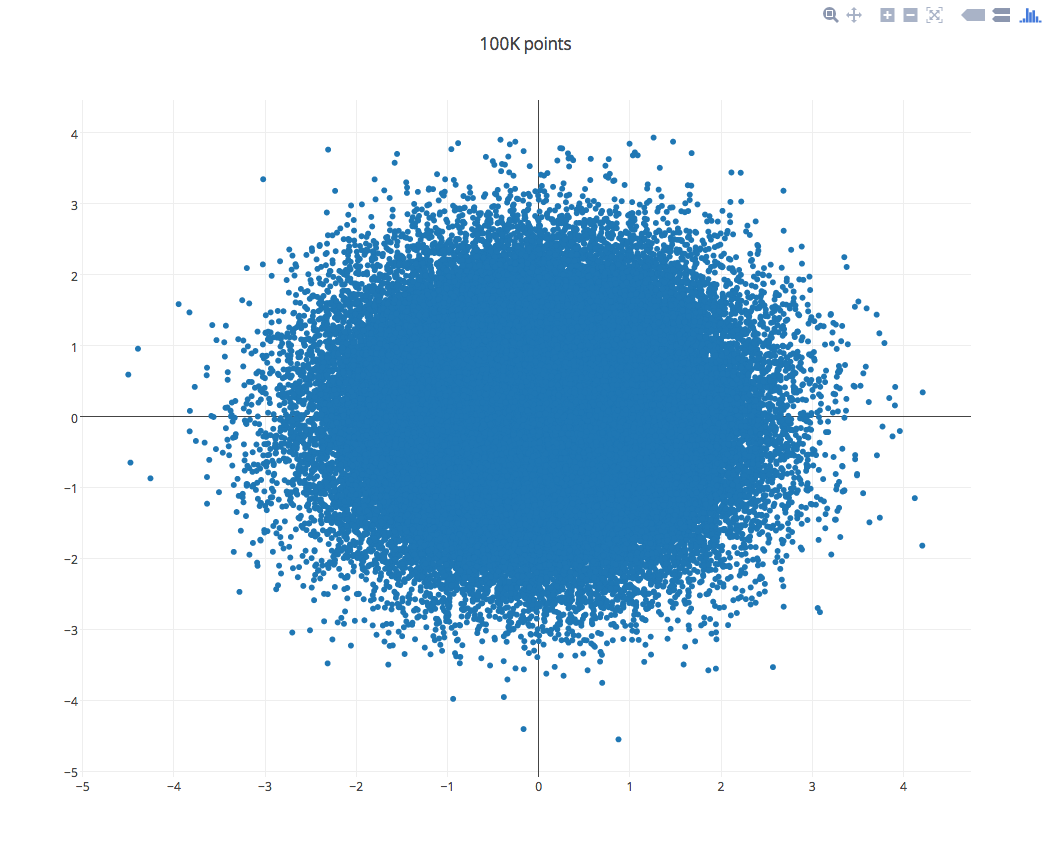
\includegraphics[scale=0.3]{scatter.png}
    \caption{A scatter plot of 100,000 points in 2D.}
    \label{scatter}
  \end{center}
\end{figure}

\begin{figure}[hbt]
  \begin{center}
    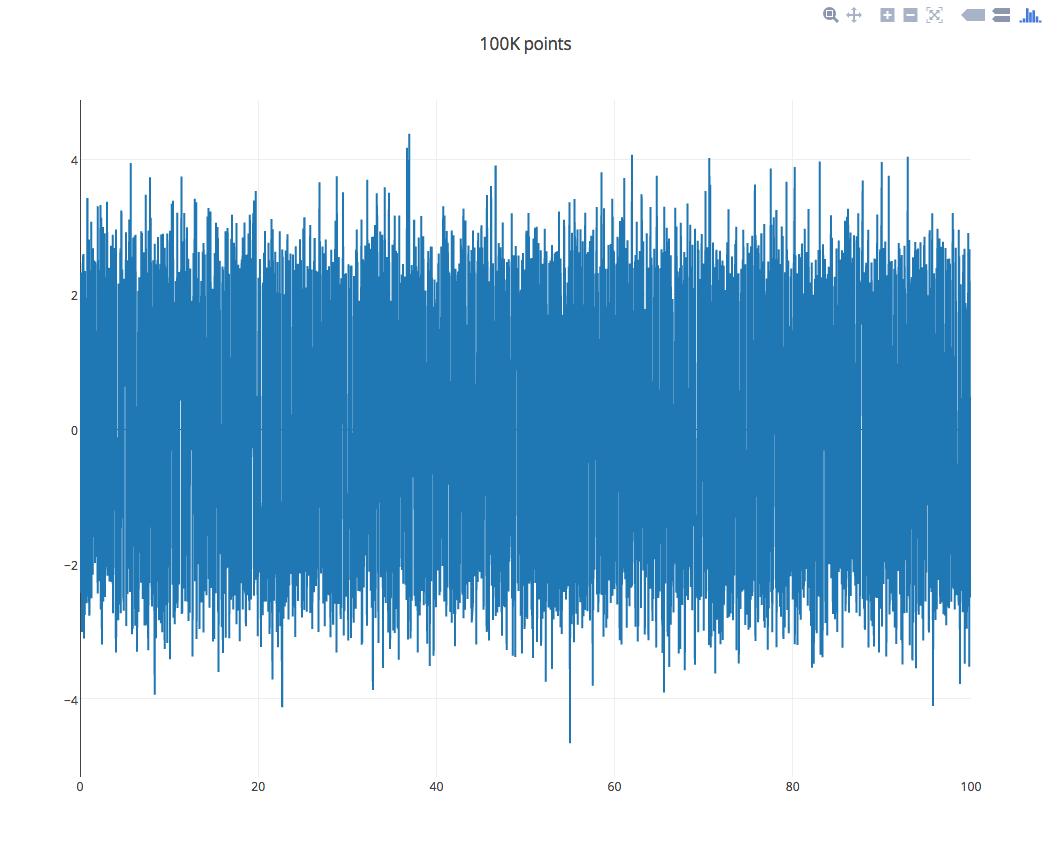
\includegraphics[scale=0.3]{line.png}
    \caption{A line plot of 100,000 points in 2D.}
    \label{line}
  \end{center}
\end{figure}

Let $P=\{p_0, p_1, \dots, p_n\}$ be a set of primitives with $p_i \in \mathbb{R}^2$ for all $i=0,1,\dots,n$.
Let $s_0 > s_1 > \dots > s_k$ be a set of scales (in our case, pixel sizes).
The \emph{cover order} of $P$ is the filtration
$$F_0 \subseteq F_1 \subseteq \dots \subseteq F_k = P$$
such that $\cup P \subseteq \cup (F_j \oplus C_{s_j})$ for each $j = 0, 1,\dots k$, where $C_{s_j}$ is a circle of radius $s_j$.
The \emph{level} of a primitive $level(p_i) = \displaystyle min_{p_i \in F_j} j$.
In other words, given a pixel size $s_j$, we would like to determine a subset of object $P' \subseteq P$ such that 
every primitive overlaps with one or more primitive of $P'$ dilated by the circle of radius $s_j$ 
(ideally, we want the minimum number of objects that would cover all others). 
This means that for a fixed zoom level, we only need to render the primitives in $P'$ as all other primitives
are ``hidden''.
%
Therefore, given a set of points/line segments, our problem can be reduced to the problem of finding a cover
order of these primitives for a given zoom level.
%Clearly, finding the cover order of a set of primitives for a given scale reduces the number of primitives the GPU needs to render. 


For pointsets in 2D, a cover order can be easily computed by the use of a spacial data structure called \emph{quadtrees}; 
however, computing a cover order is not so evident in the case of line plots. %, as we will see in the following sections. 

In what follows, we describe a method that will allow us to render and process a scatter plot of 100 million points
within a browser. % by using a simple spacial data structure called a \emph{quadtree}. 
We then discuss the challenges of using the same technique for rendering scatter plots
and propose a few possible alternatives.

\iffalse
Motivation: How can we reduce the number of curves that need to be rendered, while preserving the exact image of the plot?

Variants:
Warm up: Suppose that the marker shape is a circle with constant radius.
Allow the radii of the markers to vary. 
Allow the marker shape to vary (crosses, stars, etc.). 
Allow the marker colors to vary.
Allow the markers to have borders of different colors
Suppose the markers are partially transparent. It is possible to compute a minimal set of arcs which will render correct opacity?

WebGL: We have the following general questions to investigate:
How should we support prioritized/progressive loading?
What is the best way to implement user interactivity and selections?
How should transparent shapes be handled?

Line plots:

Definition: A line plot is a piecewise linear curve. 

Note: We currently use a min/max decimation algorithm that gives us better performance than scatter plots. 
\fi


\section{Progressive Loading of 2D Scatter Plots}

In this section we describe an algorithm that allows us to render 100 million points.
The key idea behind the algorithm is the use of the quadtree data structure,
and the building of this data structure in a way that minimizes the use of working memory. 


A \emph{quadtree} of a set of points in the plane is a geometric data structure that is constructed by recursively splitting the 
area (usually the square bounding box of the input pointset) into four equal-sized squares
until every square contains at most one point~\cite{quadtrees74}.

Let $A$ be a set of $n$ points in the plane, and let $z$ be a zoom level 
(which is a function of the current pixel size and screen resolution/size).  %(represented by their $x$ and $y$ coordinates). 

\paragraph{Preprocessing. } 
Once the points $A$ are loaded in the client (we will assume $A$ is an array of points), we preprocess them as follows.
\begin{enumerate}
\item Construct a quadtree of the pointset $A$ using a depth-first traversal of the points and 
	storing the level of each point in the quadtree in a new array $L$. 
	Store the points in array $Q$.  Thus, the level of point $Q[i]$ is stored $L[i]$.
\item Sort the points of $Q$ in increasing order of level and of x-coordinate using an in-place sorting algorithm (such as Quicksort).
	The size of array $L$ will be equal to the height of the quadtree.
\end{enumerate}

For a given zoom level $z$, this ordering of points by level gives us a way to decide which points need to be rendered
and which do not because they are ``hidden'' by others. 
Consider a square area of the quadtree, which corresponds to a node $p$ at some level $l$ in the tree. 
If the zoom level of the rendering matches with $l$, then the quadtree structure tells us that all vertices in that single square area 
will be mapped on top of each other on the screen in the final rendering on the screen. 
Therefore, instead of rendering all the points ($p$ and its descendants), we can instead render only point $p$. 


\paragraph{Rendering. } 
Once array $Q$ is constructed and sorted, we can now flush array $L$ and send $Q$ to the GPU.
To render for a given level, we ask the GPU to draw some superset of the points that are visible on the
screen and are not hidden behind others.

\begin{enumerate}
\item Compute the size of a pixel in the data coordinate to get the current zoom level $z$.
\item Compute the $x_{min}$ and $x_{max}$ of the screen.
\item Starting at level $z$, for each level above $z$
	\begin{enumerate}
		\item Find the predecessor $x_p$ of $x_{min}$ and successor $x_s$ of $x_{max}$.
		\item Ask the GPU to draw the points whose $x$-coordinates are between $x_p$ and $x_s$.
	\end{enumerate}
\end{enumerate}



\begin{figure}[hbt]
  \begin{center}
    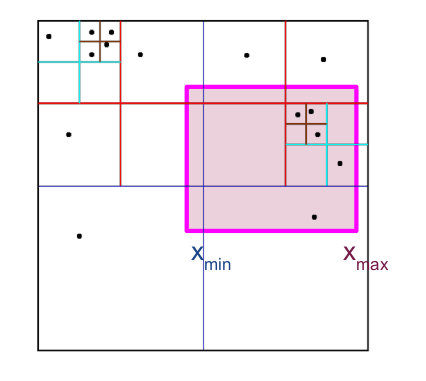
\includegraphics[scale=0.6]{quadtree-screen.png}
    \caption{The partitioning of the points into quadtree partitions. The pink/bold rectangle represents the area that will appear on the screen.}
    \label{quad}
  \end{center}
\end{figure}


Conceptually, given a zoom level $z$, we will ask the GPU to draw all the points that have level \emph{at most} $z$, thus ignoring
all points that are deeper than $z$ in the quadtree. 
We further trim the number of rendered points by excluding the ones that are outside the vertical strip 
that encloses that sides of the screen. See Figure~\ref{quad}.

%For each zoom level, this ordering of the points by level gives us a way to decide which points need to be rendered, and which do not because they are overshadowed by others. Thus, if the user zooms to level k, then the points that need to be rendered are the ones that have level at most k in the quadtree. Hence, the only points that need to be sent to the GPU for rendering are the points Q[0], Q[1], …, Q[L[k+1]-1]. 

\paragraph{Analysis.}

Preprocessing may take a long time if the quadtree ends up having height O(n).
● This happens when the input consists of a big
cluster of points that are far from the rest of the
points.
● To avoid such a bad case, we introduce a small
change to the way we construct the quadtree.

A quadtree of depth $d$ storing a set of $n$ points has $O((d + 1)n)$ nodes and can be constructed in $O((d + 1)n)$ time.
In general, the depth of a quadtree of a set of points in the plane is at most $\log (s/c) + \frac{3}{2}$, 
where $s$ is the length of one the edges of the bounding box and $c$ is the distance between 
the closest pair of points. Thus, in the worst case, the depth of a quadtree can be arbitrarily bad. 

Preprocessing may take a long time if the quadtree ends up having height $(n)$.
This happens when, for example, the input consists of a big cluster of points that are far from the rest of the
points. To avoid such bad cases, we introduce a slight modification to the way we construct the quadtree:
After every split of the area into four quadrants, we check each quadrant to see if any contains greater
than 90\% of the points. If such a quadrant is found, then split the point cluster arbitrarily into two equal sets and
construct a new quadtree for each one separately.
Doing this will preserve the level information for each point, which is all that we need to render effectively,
while at the same time decreasing the height of the tree.

The algorithm described in this section has made it possible to render 100 million points inside a browser while maintaining
reasonable interactivity of the plot.



\paragraph{A note on transparent markers of the same color and shape.}

So far we have assumed that the markers we are rendering are of solid color. 
This assumption made it possible to replace all points that are stacked on top of each other 
with a single point on the screen.
If the markers are partially transparent however, replacing overlapping points with a single, equally-transparent marker
will not work as we need to blend the colors of all the markers that are hidden. 
Blending different colors assumes an ordering of the points, which makes the problem even more complex.
Here we propose a simple fix to the case of partially transparent markers that have the same color and shape. 
To blend colors properly, we need to know the number of points hidden behind the point we want to render. 
We can save this information while creating the quadtree in the preprocessing step --- for each 
node of the quadtree, we keep track of the number of descendants in its subtree and 
store this number in a separate array. 
While rendering, we can then use this information to blend the colors appropriately. 




\section{Progressive Loading of 2D Line Plots}



[1] R. A. Finkel and J. L. Bentley. Quad trees: a data structure for retrieval on composite keys. Acta Inform., 4:1–9, 1974.

\vskip2cm

\section*{Acknowledgements}
We would like to thank the participants and organizers of the \emph{Sixth Montreal Industrial Problem Solving Workshop}
where the problem was first posed. 

\end{document}
